\section{Background, Examples, \& Goals}

A single top-level web page often incorporates multiple scripts
written by different authors.\footnote{Throughout we use ``web page''
  and ``web application'' interchangeably, and ``JavaScript code'' and
  ``script'' interchangeably.}
%\Red{EZY suggests cutting:
Ideally, the browser should protect the
user's sensitive data from unauthorized disclosure, yet afford page
developers the greatest possible flexibility to construct %richly
featureful applications that reuse functionality implemented in
scripts provided by (potentially untrusted) third parties. To make
concrete the diversity of potential trust relationships between
scripts' authors and the many ways page developers structure
amalgamations of scripts, we describe several example web
applications, none of which can be implemented with strong privacy for
the user in today's web browsers. These examples illustrate key
requirements for the design of a flexible browser confinement
mechanism. Before describing these examples, however, we offer a brief
refresher on status-quo browser privacy polices.
% and a sketch of the labeling mechanism that
%forms the core of our system, \sys{}.

\subsection{Browser Privacy Policies}
%%Contexts and the Same-Origin Policy}
\label{sec:backgd}

\paragraph{Browsing contexts}
\begin{figure}
\begin{center}
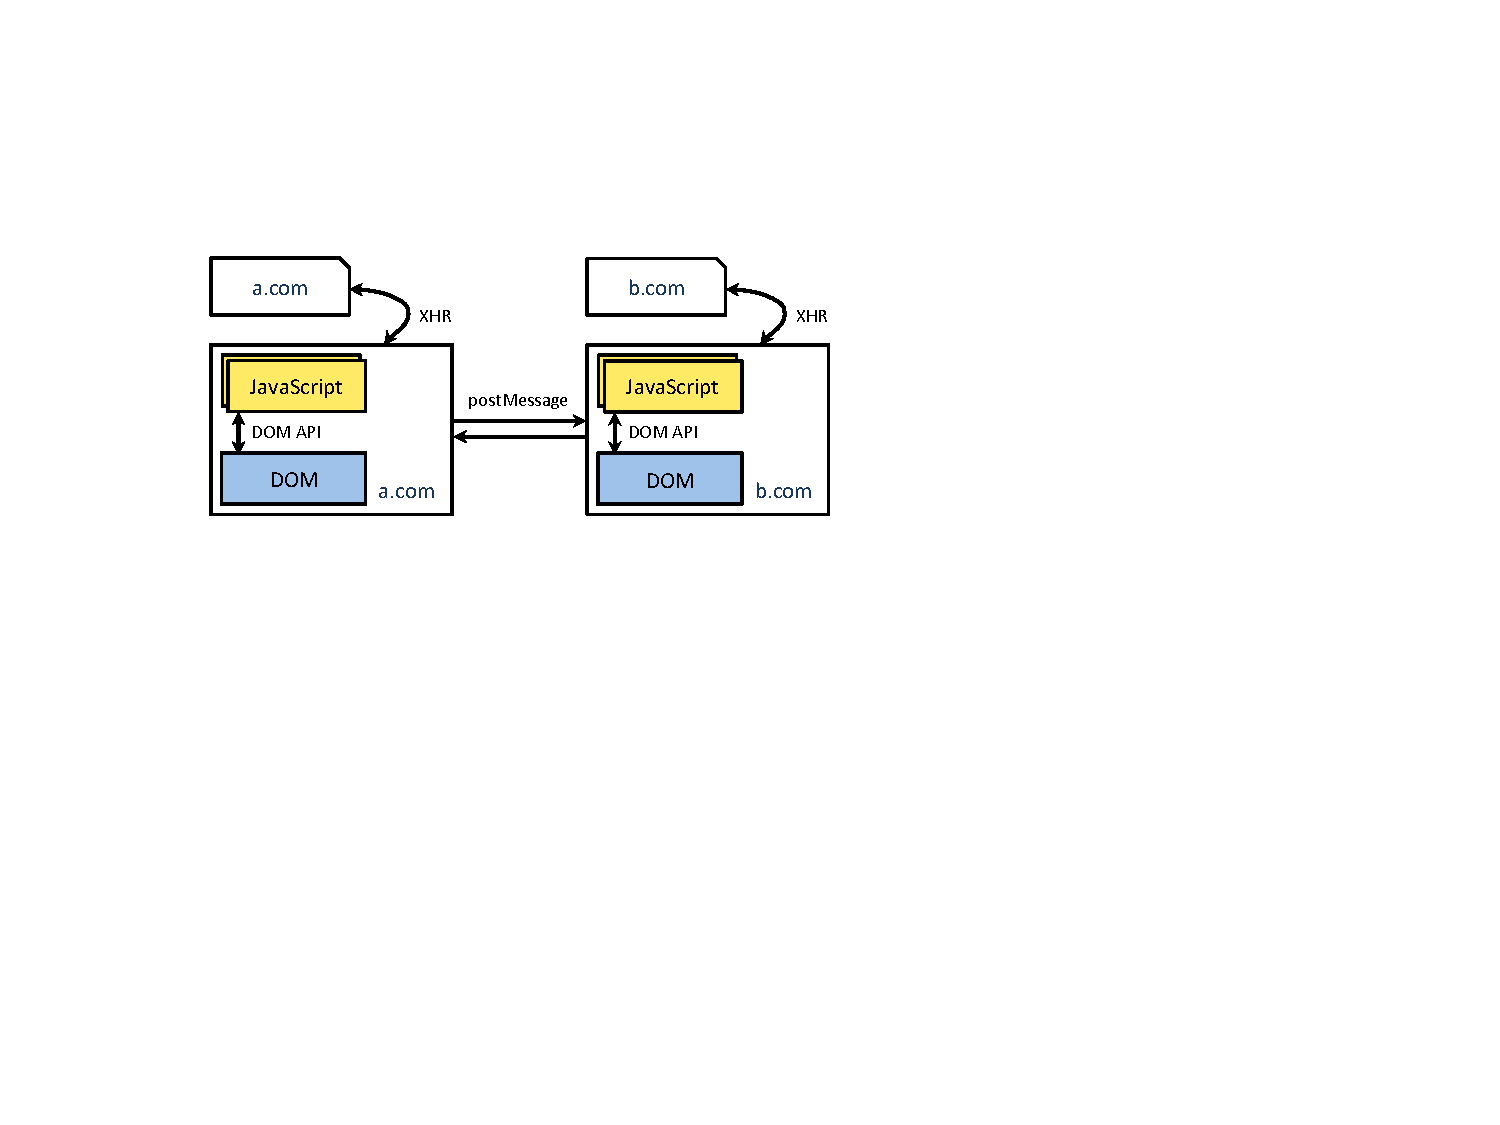
\includegraphics[width=\columnwidth]{arch.pdf}
%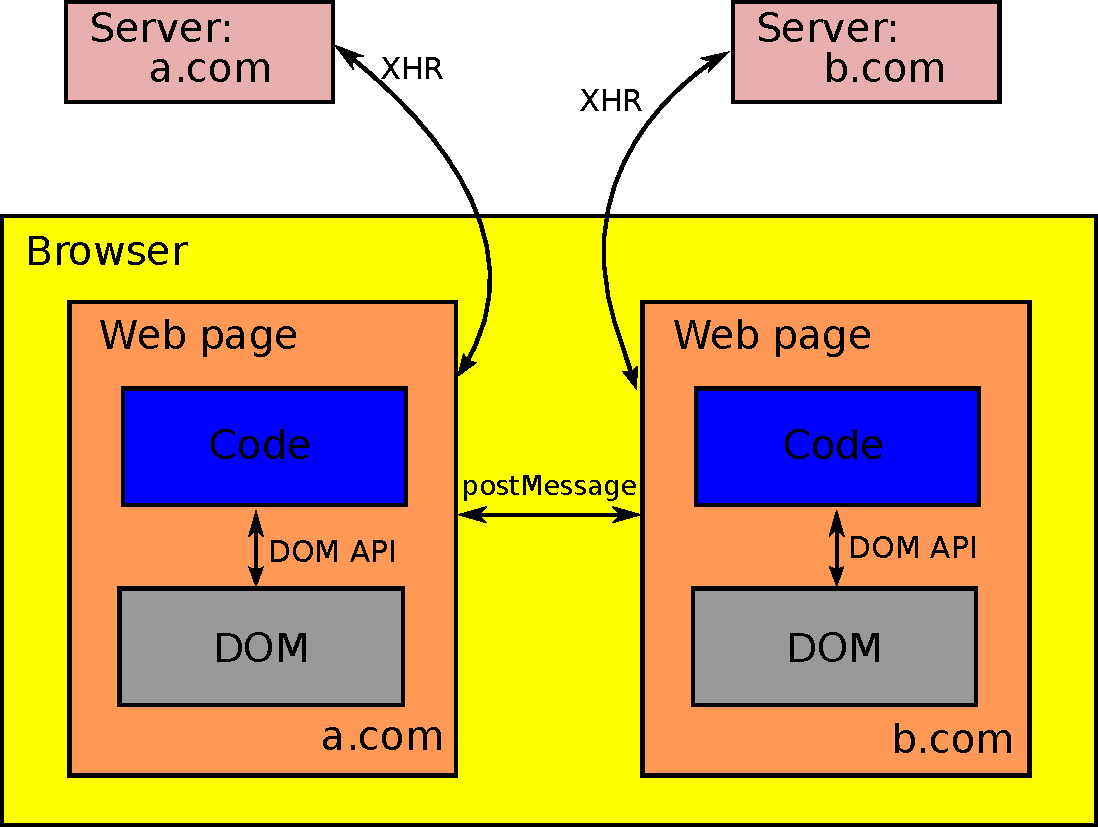
\includegraphics[scale=0.35]{setting.pdf}
\end{center}
\vspace{-10pt}
\caption{\label{fig:primer-browser-arch} Simplified browser
architecture.}
%\vspace{-5pt}
\end{figure}
Figure~\ref{fig:primer-browser-arch} depicts the basic building blocks of
the current web security architecture.
%
%% Core to this design is the notion of \emph{browsing
%% contexts}, \emph{i.e.,} pages and frames.
%
A \emph{browsing context} (\emph{e.g.,} a page or frame) encapsulates
presentable content and a JavaScript execution environment (heap and
code) that interacts with content through the \emph{Document Object
  Model (DOM)}~\cite{html5}.
%
Browsing contexts may be nested (\emph{e.g.,} by using iframes).
%
They also may read and write persistent storage (\emph{e.g.,} cookies), issue
network requests (either implicitly in page content that references a
URL retrieved over the network, or explicitly in JavaScript, using the
\xhr{} (XHR) constructor), and communicate with other contexts
(IPC-style via \js|postMessage|, or, in certain cases, by sharing
DOM objects).
%
Some contexts such as Web Workers~\cite{workers} run JavaScript but do not instantiate a
DOM. We use the terms \emph{context} and \emph{compartment}
interchangeably to refer to both browsing contexts and workers, except when
the more precise meaning is relevant.

\paragraph{Origins and the Same-Origin Policy}
Since different authors may contribute components within a page,
today's status quo browsers impose a security policy on interactions
among components. Policies are expressed in terms of \emph{origins}.
An origin is a source of authority encoded by the protocol (\emph{e.g.,}
\js|https|), domain name (\emph{e.g.,} \js|fb.com|), and port (\emph{e.g.,} \js|443|)
of a resource URL. For brevity, we elide the protocol and
port from URLs throughout.

The same-origin policy specifies that an origin's
resources should be readable only by content from the same
origin~\cite{rfc6454, googlehandbook, VanKesteren2012}.  Browsers
ensure that code executing in an \https{a.com} context can only
inspect the DOM and cookies of another context if they share the same
origin, \emph{i.e.,} \https{a.com}. Similarly, such code can only
inspect the response to a network request (performed with XHR) if the
remote host's origin is \https{a.com}.
%
%% In general, the SOP isolates code in one page from accessing client-
%% and server-side data associated with another origin.
 
The SOP does not, however, prevent code from \emph{disclosing} data to
foreign origins. For example, code executing in an \https{a.com}
context can trivially disclose data to \https{b.com} by using XHR to
perform a network request; the SOP prevents the code from
inspecting responses to such cross-origin XHR requests, but does not
impose any restrictions on sending such requests.
Similarly, code can exfiltrate data by encoding it in the path of a
URL whose origin is \https{b.com}, and setting the \js|src| property
of an \js|img| element to this URL.

\paragraph{Content Security Policy (CSP)}

Modern browsers allow the developer to protect a user's privacy by
specifying a CSP that limits the communication of a page---\emph{i.e.,}
that disallows certain communication ordinarily permitted by the SOP\@.
Developers may set individual CSP directives to restrict the origins
to which a context may issue requests of specific types (for images or
scripts, XHR destinations, \emph{etc.})~\cite{csp}. However, CSP policies
suffer from two limitations. They are {\em static:} they
cannot change during a page's lifetime (\emph{e.g.,} a page may not
drop the privilege to communicate with untrusted origins before
reading potentially sensitive data). And they are {\em inaccessible:}
JavaScript code cannot inspect the CSP of its enclosing context or
some other context, \emph{e.g.,} when determining whether to share
sensitive data with that other context.

%% To improve user privacy developers can use CSP to impose additional
%% policies on a context.
%% %
%% Specifically, with CSP, developers can set various directives to
%% restrict the origins from where different content (images, scripts,
%% \emph{etc.}) may be loaded~\cite{csp}.
%% %
%% While the initial intent of this was to address cross-site scripting
%% (XSS) attacks by limiting code to be loaded from trustworthy sources,
%% CSP evolved to address a broader class of privacy issues, including
%% (explicit) exfiltration.
%% %
%% For instance, the fine-grained control over resource loading has the
%% dual purpose of restricting to whom data can be leaked through content
%% loading.
%% %
%% (If a page is restricted to only including images from \https{b.com},
%% it can only leak data through image loading to this (\emph{i.e.,}
%% \https{b.com}) origin.)
%% %
%% Other CSP directives have the sole role of preventing leaks.
%% %
%% For example, the \texttt{connect-src} directive is used to white-list
%% the origins that a page is allowed to communicate with via XHR.

%% Unfortunately, CSP cannot be used to restrict certain channels such as
%% inter-compartment messaging (\emph{e.g.,} via \js|postMessage|) or leaks due
%% to navigation.
%% %
%% This, however, is not a fundamental limitation of CSP and indeed
%% within the scope of future versions of the specification~\tocite{}.
%% %
%% More fundamentally, CSP policies are 1) \emph{static}, \emph{i.e.,} policies
%% cannot change through the lifetime of a page (\emph{e.g.,} a page cannot drop
%% communication privileges with certain hosts); and 2)
%% \emph{inaccessible}: JavaScript code cannot inspect the CSP policy of
%% its context, or the policy of another context when, for instance,
%% deciding to share sensitive data with the latter party.

\paragraph{postMessage and Cross-Origin Resource Sharing (CORS)}

As illustrated in Figure~\ref{fig:primer-browser-arch}, the
HTML5 \js|postMessage| API~\cite{webmessaging} enables cross-origin
communication in IPC-like fashion within the browser. To prevent
unintended leaks~\cite{barth2009securing}, a sender always
specifies the origin of the intended recipient; only a context with
that origin may read the message.
%
%% When sending a message, the sender can specify intended origin of the
%% to ensure that an arbitrary context cannot read the message.
%
%% Otherwise, a malicious attacker may be able to carry out a
%% man-in-the-middle attack by navigating the context to whom the message
%% was destined for to a page they control (wherein they read the
%% message)~\cite{barth2009securing}.

%%\todo{}{It would be better to emphazise who sets CORS. What about:
%%  CORS~\cite{cors13} goes a step further, and allows web servers to extend the
%%  (cross-) domains capable to observe its responses. Under CORS, a server may
%%  include a header on returned content that explicitly whitelists other
%%  origin(s) to read its responses.\footnote{Recall that the default SOP blocks a
%%    context from reading a response from a different origin.}  }

CORS~\cite{cors13} goes a step further and allows controlled
cross-origin communication between a browsing context of one origin
and a remote server with a different origin. Under CORS, a server may
include a header on returned content that explicitly whitelists other
origin(s) allowed to read the response.
%%\footnote{Recall that the default SOP
%%  blocks a context from reading a response from a different origin.}

%
%% Specifically, with CORS, code can read cross-origin resources,
%% retrieved via XHR, if the remote host supplies a CORS header
%% white-listing the (requesting) origin, alongside the resource.
%% %
%% Recall that the SOP would otherwise disallow code from inspecting a
%% cross-origin response.
 
Note that both \js|postMessage|'s target origin and CORS are purely
discretionary in nature: they allow static selection of which
cross-origin communication is allowed and which denied, but enforce no
confinement on a receiving compartment of differing origin. Thus, in
the status-quo web security architecture, a privacy-conscious
developer should only send sensitive data to a compartment of
differing origin if she completely trusts that origin. 

%% are solely a form of discretionary access control.
%% %
%% They give the sending compartment or server control over the origins
%% that are allowed to read the resource/message, but once access is
%% granted, they have no control over what the cross-origin compartment
%% can do with the data.
%
%% Hence in the status quo, a developer should only send sensitive data
%% to a cross-origin compartment if she completely trusts the foreign
%% origin.

\subsection{Motivating Examples}
\label{sec:motivating-examples}

Having reviewed the building blocks of security policies in status-quo
web browsers, we now turn to examples of web applications for which
strong privacy is not achievable today. %the status quo. 
These examples
illuminate key design requirements for the \sys{} confinement
system. %, as well as the overall intuition behind its design.

\paragraph{Password Strength Checker} Given users' propensity for choosing poor
(\emph{i.e.,} easily guessable) passwords, many web sites today incorporate
functionality to check the strength of a password selected by a user
and offer the user feedback (\emph{e.g.,} ``too weak; choose another,''
``strong,'' \emph{etc.}). Suppose a developer at Facebook (origin
\js|fb.com|) wishes to re-use password-checking functionality provided
in a JavaScript library by a third party, say, from origin
\js|sketchy.ru|. If the developer at \js|fb.com| simply includes the
third party's code in a \js|script| tag referencing a resource at
\js|sketchy.ru|, then the referenced script will have unfettered
access to both the user's password (provided by the Facebook page,
which the library {\em must} see to do its job) and to write to the
network via XHR\@. This simple state of affairs is emblematic of the
ease with which na\"{\i}ve web developers can introduce leaks of
sensitive data in applications.

A more skilled web developer could today host the checker script on
her {\em own} server and have that server specify a CSP policy for the
page.
%
Unfortunately, a CSP policy that disallows scripts within the page
from initiating XHRs to any other origins is \emph{too inflexible,} in
that it precludes useful operations by the checker script, \emph{e.g.,}
retrieving an updated set of regular expressions describing weak
passwords from a remote server (essentially, ``updating'' the
checker's functionality). Doing so requires communicating with a
remote origin.
%
Yet a CSP policy that permits such communication, even with the
top-level page's same origin, is \emph{too permissive:} a malicious
script could potentially carry out a \emph{self-exfiltration attack}
and write the password to a public part of the trusted
server~\cite{Yip:2009:PBS, selfex}.

This trade-off between flexibility and privacy, while inherent to
CSP, need not be fundamental to the web model.
%
The key insight is that it is entirely safe and useful for an untrusted script to
communicate with remote origins {\em before} it reads sensitive
data. We note, then, the requirement of a confinement mechanism that
allows code in a compartment to communicate with the network {\em
  until it has been exposed to sensitive data.} MAC-based confinement
meets this requirement.

\begin{figure}
\centerline{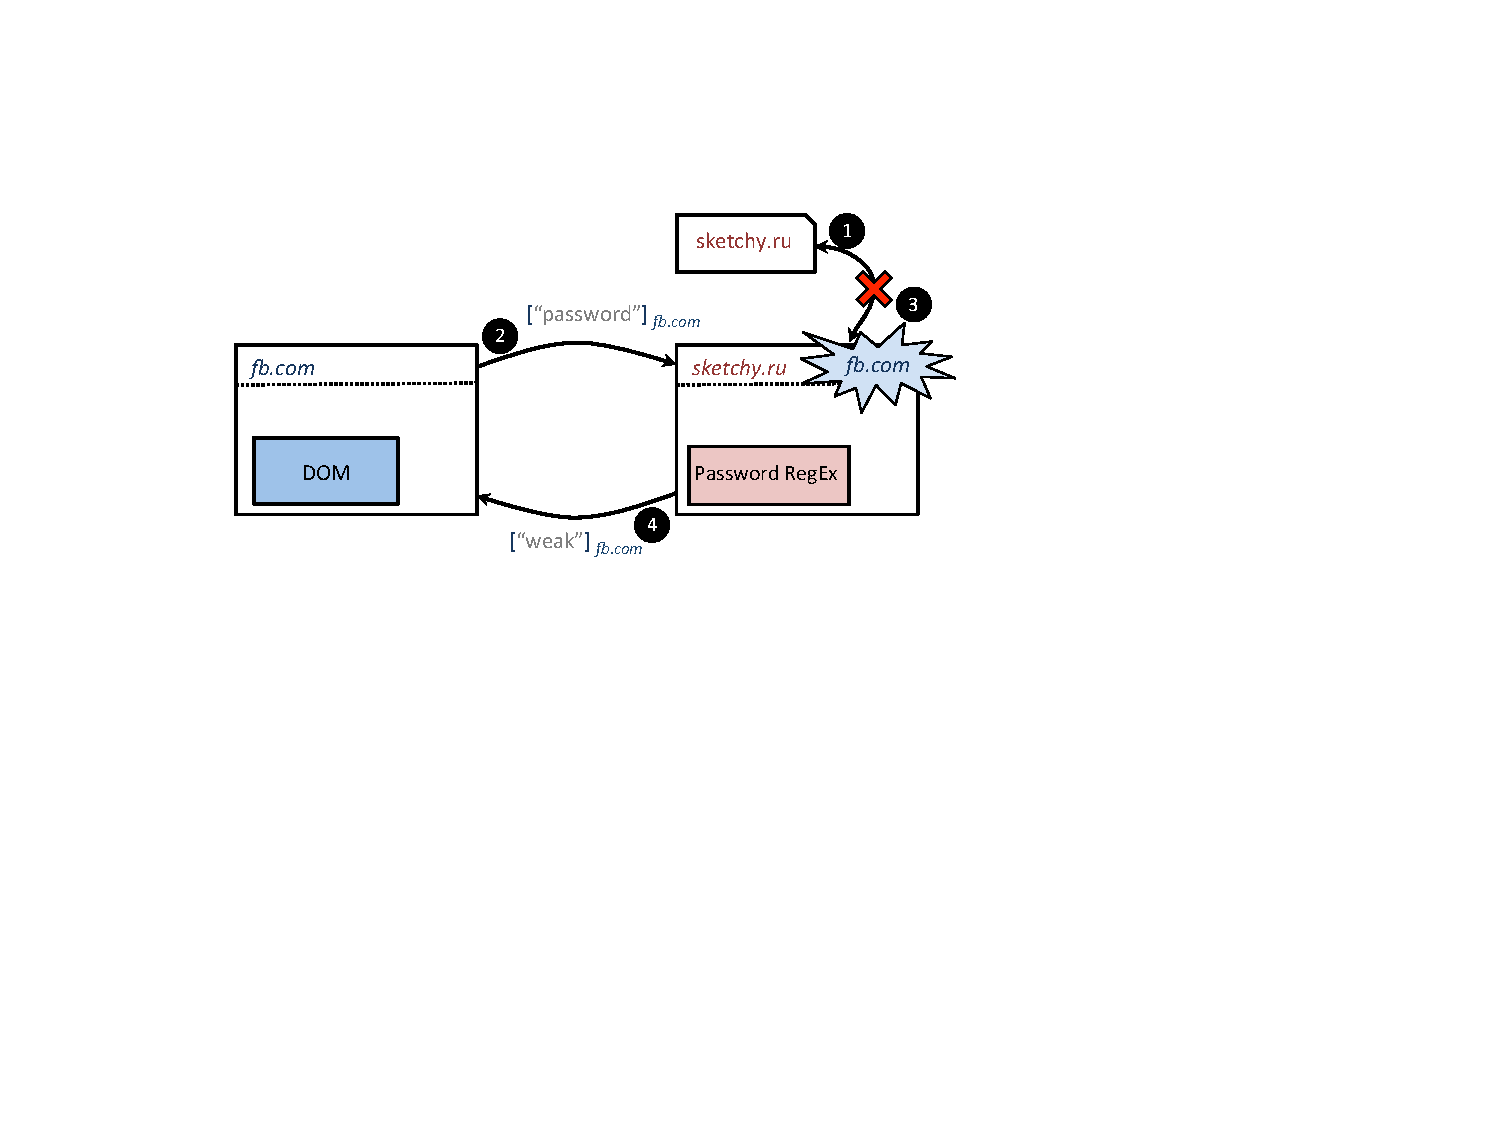
\includegraphics[width=\columnwidth]{checker}}
\caption{\label{fig:checker} Third-party password checker architecture
under \sys{}.}
\end{figure}

Figure~\ref{fig:checker} shows how such a design might look. In this
and subsequent examples, rectangular frames denote compartments,
arrows denote communication (either between a compartment and the
network, or IPC-style between compartments), and events during
execution are numbered sequentially in time. As we have proposed
previously~\cite{yang:2013:towards}, compartments may be
\emph{labeled} (Section~\ref{sec:system:contexts}) with the origins to
whose sensitive data they have been exposed. A compartment that has
not yet observed sensitive data is denoted \js|public|; however, when
it wishes to incorporate sensitive data, the compartment \emph{raises}
its label (at the cost of being more restricted in where it can
write). We illustrate the raising of a label with a ``flash''
connoting the sensitivity of data being integrated.  A compartment's
\emph{privilege} (Section~\ref{sec:system:privileges}), which specifies the
origins for which a script executing in that compartment is trusted,
is indicated by a crown. Here, a top-level page at \js|fb.com|
encapsulates a password-checker script from a third-party origin in a
new compartment. The label of the new compartment is initially
\js|public|.
%%\todo{}{Here, it would be clearer to refer explicitly to the message, \emph{e.g.,} 
%%``In step (2), the top-level page sends the user's password to 
%%the checker script's worker, denote by the message $[``password'']_{fp.com}$---
%%we ignore the messages subindexes (to be explained in Section XXX)''}
%%\todo{}{We need to describe better what is a label and a privilege in the
%%  picture. A bit confusing with the underline. The crown is a good idea}
First, in step (1), the checker script is free to
download updated regular expressions from an arbitrary remote
origin. In step (2), the top-level page sends the user's password to
the checker script's worker using \js|postMessage|; the password is
\emph{labeled} \js|fb.com| to indicate that the data is sensitive to
this origin (Section~\ref{sec:system:communication}).
%
%%When the browser delivers the password to the checker
%%script's context, it raises the label of the context to reflect that
%%the context is about to be exposed to sensitive data from \js|fb.com|. 
%
In step (3) the checker raises its label to reflect that the context
is about to be exposed to sensitive data from \js|fb.com| and
inspects the password.
%
When the label is raised, \sys{} atomically denies the context further
access to the network in step (3).\footnote{
  For clarity, we use \texttt{fb.com} as the label on the data.  This
  label still allows the checker to send XHR requests to
  \texttt{fb.com}; to ensure that the checker cannot communicate with
  \emph{any} origin, COWL provides fresh origins (see
  Section~\ref{sec:system:privileges}).
}
%
However, the checker script is free to compute the result, which
it then returns via \js|postMessage| to the top-level page in step (4); the
result carries the label \js|fb.com| to reflect that the sender may be
sending data derived from sensitive data owned by \js|fb.com|.
%
Since the top-level page has the \js|fb.com| privilege, it can simply
read the data (without raising its label).
% bk: unneeded to clutter this first simple example with the below, as
% other examples illustrate the need for hierarchical confinement?
%  We note further the requirement of a {\em hierarchical}
% confinement mechanism: the checker script may itself invoke untrusted
% code from still {\em other} third-party origins, and should be able to
% further confine such untrusted code.

\paragraph{Encrypted Document Editor}
%% XXX IMPORTANT bk:
%% need to articulate usage model as *company* wants to encrypt its
%% documents stored in Google Docs, and that *company* writes the
%% encryption code, which is hosted from its origin. This eliminates
%% objection, "why would the user trust the encryption library to
%% encrypt correctly, but *not* trust it not to leak the cleartext?"
Today's web applications, such as in-browser document editors backed
by cloud-based storage (\emph{e.g.,} Google Docs), typically require the user
to trust the app developer/cloud-based storage provider (often the
same principal under the SOP) with the data in her documents. That is,
the provider's server observes the user's data in cleartext. Suppose
an organization wished to use an in-browser document editor but did
{\em not} want to reveal its users' document data to the editor
provider's server. How might the provider offer a privacy-preserving
editor app that would satisfy the needs of such a privacy-conscious
organization?  One promising approach might be for the ``customer''
privacy-sensitive organization to implement a trusted document encryption
service hosted at its own origin, distinct from that which hosts the
editor app. The editor app could allow the user to specify a JavaScript
``plugin'' library she trusts to perform cryptography correctly. In this design,
one origin serves the JavaScript code for the editor app (say,
\js|gdocs.com|) and a different origin serves the JavaScript code for
the cryptography library (say, \js|eff.org|). Note that these two
origins may be {\em mutually distrusting.}
\js|gdocs.com|'s script must pass the document's cleartext to a script
from \js|eff.org| for encryption, but would like to confine the
execution of the encryption script so that it cannot exfiltrate the
document to any origin {\em other} than \js|gdocs.com|. Similarly,
\js|eff.org|'s cryptography library may not trust \js|gdocs.com| with
the cleartext document---it would like to confine \js|gdocs.com|'s
editor to prevent exfiltration of the cleartext document to
\js|gdocs.com| (or to any other origin).
%
This simple use case highlights the need for {\em
  symmetric confinement:} when two mutually distrusting scripts from
different origins communicate, {\em each must be able to confine the
  other's further use of data it provides.}
%
%% XXX ds: want to use "at the end of the day;" too colloquial?
%% Moreover, since it is in the interest of both parties to actually
%% store the encrypted document, it is important for the confinement
%% system to support {\em declassification}: \js|gdoc.com| should be
%% allowed to store encrypted documents provided by \js|eff.org|.

%% brings up the requirement of *symmetric* confinement: two mutually
%% distrusting origins each confine the other.

\paragraph{Third-Party Mashup}
Some of the most useful web applications are {\em mashups}; these
applications integrate and compute over data hosted by multiple
origins. For example, consider an application that reconciles a user's
Amazon purchases (the data for which are hosted by \js|amazon.com|)
against a user's bank statement (the data for which are hosted by
\js|chase.com|). The user may well deem both these categories of data
sensitive and will furthermore not want data from Amazon to be
exposed to her bank or vice-versa, nor to any other remote party.
Today, if one of the two providers implements the mashup, its
application code must bypass the SOP to allow sharing of data across
origin boundaries, \emph{e.g.,} by communicating between iframes with
\js|postMessage| or setting a permissive CORS policy.  This approach
forfeits privacy: one origin sends sensitive data to the other, after
which the receiving origin may exfiltrate that sensitive data at will.
Alternatively, a third-party developer may wish to implement and offer
this mashup application. Users of such a {\em third-party mashup} give
up their privacy, usually by simply handing off credentials, as again
today's browser enforces no policy that confines the sensitive data
the mashup's code observes within the browser. To enable third-party
mashups that do not sacrifice the user's privacy, we note again the
need for an untrusted script to be able to issue requests to multiple
remote origins (\emph{e.g.,} \js|amazon.com| and \js|chase.com|), but
to lose the privilege to communicate over the network once it has read
the responses from those origins. Here, too, MAC-based confinement
addresses the shortcomings of DAC. 

\paragraph{Untrusted Third-Party Library}
Web application developers today make extensive use of third-party
libraries like jQuery. Simply importing a library into a page provides
no isolation whatsoever between the untrusted third-party code and any
sensitive data within the page. Developers of applications that
process sensitive data want the convenience of reusing popular
libraries. But such reuse risks exfiltration of sensitive data by
these untrusted libraries. Note that because jQuery requires access to
the content of the entire page that uses it, we cannot isolate jQuery
in a separate compartment from the parent's, as we did for the
password-checker example. Instead, we observe that jQuery demands a
design that is a mirror image of that for confining the password
checker: we place the {\em trusted} code for a page in a separate
compartment and deem the rest of the page (including the untrusted
jQuery code) as untrusted. The trusted code can then communicate with
remote origins and inject sensitive data into the untrusted page, but
the untrusted page (including jQuery) cannot communicate with remote
origins (and thus cannot exfiltrate sensitive data within the
untrusted page).
%% Once more, MAC-based confinement intuitively seems to
%% fit this scenario well.
This refactoring highlights the need for a confinement system that
supports {\em delegation} and {\em dropping privilege}: a page should
be able to create a compartment, confer its privileges to
communicate with remote origins on that compartment, and then give
these privileges up.

We note further that any {\em library} author
may wish to reuse functionality from another untrusted
library. Accordingly, to allow the broadest reuse of code, the browser
should support {\em hierarchical confinement}---the primitives for
confining untrusted code should allow not only a single level of
confinement (one trusted context confining one untrusted context), but
arbitrarily many levels of confinement (one trusted context confining
an untrusted one, that in turn confines a further untrusted one,
\emph{etc.}).

%% describe trusted compartment between page w/JQuery and network as
%% firewall---its job is to deny network requests to origins other
%% than those that are trusted.

%% after discussion with Deian:
%% there are two versions of this scenario.
%%
%% (1) page initially includes sensitive data. so steps are:
%%      (a) page creates worker with DOM access and privilege
%%      (b) page raises label to a.com; hereafter page cannot talk to
%%      any origin but a.com (so cannot leak elsewhere).
%%      (c) tcb code (in worker) loads jquery and injects it into page
%%      (d) jquery is now in page, and cannot leak
%%
%% (2) page initially includes no sensitive data, so steps are:
%%      (a) page has public label
%%      (b) page creates worker with DOM access and privilege
%%      (c) page drops privilege
%%      (d) page loads jquery (note label not raised yet!)
%%      (e) hereafter, page can only send to a.com and worker
%%      (f) worker only allows flows to allowed origins
%%      (g) tcb code transfers sensitive data from a.com, proxies into
%%      page
%%
%%  in both cases, untrusted jquery runs in page, but cannot leak to
%%  non-a.com origins.

\subsection{Design Goals}

We have briefly introduced four motivating web applications that
achieve rich functionality by combining code from one or more
untrusted parties. The privacy challenges that arise in such
applications are unfortunately unaddressed by status-quo browser
security policies, such as the SOP\@. These applications clearly
illustrate the need for robust yet flexible confinement for untrusted
code in browsers. To summarize, these applications would appear to be
well served by a system that:
\begin{CompactItemize}
\item Applies mandatory access control (MAC);
\item Is {\em symmetric,} \emph{i.e.,} it permits two principals to {\em
    mutually} distrust one another, and each prevent the other from
  exfiltrating its data;
\item Is {\em hierarchical, } \emph{i.e.,} it permits principal
  $A$ to confine code from principal $B$ that processes $A$'s data,
  while principal $B$ can independently confine code from principal
  $C$ that processes $B$'s data, \emph{etc.}
%% \item Supports {\em declassification,} \emph{i.e.,} it allows principal $A$
%%   to declassify data sensitive to $A$ (but, of course, not $B$);
\item Supports {\em delegation} and {\em dropping privilege,} \emph{i.e.,} it
  permits a script running in a compartment with the privilege to
  communicate with some set of origins to confer those privileges
  on another compartment, then relinquish those privileges itself.
  %% to grant another principal the ability to ``speak, '' \emph{i.e.,} 
  %% declassify and delegate, on its behalf, and revoke its own ability
  %% to do so.
  %% XXX ds: don't like "revoke its ability do do so"
\end{CompactItemize}
In the next section, we describe \sys{}, a new confinement system that
satisfies these design goals.
